\documentclass{article}
\usepackage{graphicx}
\usepackage{amsmath}
\usepackage[spanish]{babel}
\begin{document}

	\begin{titlepage}
		\centering
		\vfill
		\fbox{\Huge{Quinta práctica}} \\
		\vfill
		\large{\textsc{Hugo Tonatiuh Carrillo Bonilla}}\\
		\vfill
		320026379
		\vfill
		\begin{center}
			
\includegraphics[width=\linewidth]{./images/Portada.jpg}
		\end{center}
		\vfill
	\end{titlepage}

	\section*{Parte 1: Calculando $\pi$ a dardazos}
		\subsection*{Actividad 1.1 - Un número fijo de dardos}

			Para el ejercicio 4, definí dos variables \texttt{dardoAbcisa} y \texttt{dardoOrdenada} (elegí estos nombres porque X y Y se parecían visualmente). Después sumé sus cuadrados en una variable llamada dardo. Si esta variable era menor igual a 1, aumentaba un contador de \texttt{dardosDentro}. Esto era implementado dentro de un ciclo \texttt{while} cuyo contador se llamaba \texttt{dardos}. Esto tuvo la ventaja de que, cuando tuve que cambiar el código para que lanzara cantidades distintas de dardos, solo tuve que cambiar una variable. Al final, dividí \texttt{dardosDentro} entre \texttt{dardos}.

			Los resultados de mi programa fueron:

			\begin{table}[!ht]
			    \centering
			    \begin{tabular}{|l|l|l|}
			    \hline
				No. de Experimento & No. de Dardos & Estimación de $\pi$ \\ \hline
				1 & 100 & 3.12 \\ \hline
				2 & 100 & 3.16 \\ \hline
				3 & 100 & 3.36 \\ \hline
				4 & 1000 & 3.148 \\ \hline
				5 & 1000 & 3.076 \\ \hline
				6 & 1000 & 3.156 \\ \hline
				7 & 10000 & 3.178 \\ \hline
				8 & 10000 & 3.1692 \\ \hline
				9 & 10000 & 3.1348 \\ \hline
				10 & 100000 & 3.1422 \\ \hline
				11 & 100000 & 3.1404 \\ \hline
				12 & 100000 & 3.13232 \\ \hline
				13 & 1000000 & 3.142332 \\ \hline
				14 & 1000000 & 3.145604 \\ \hline
				15 & 1000000 & 3.142852 \\ \hline
			    \end{tabular}
			\end{table}

			Y mi captura es:

			\begin{center}
				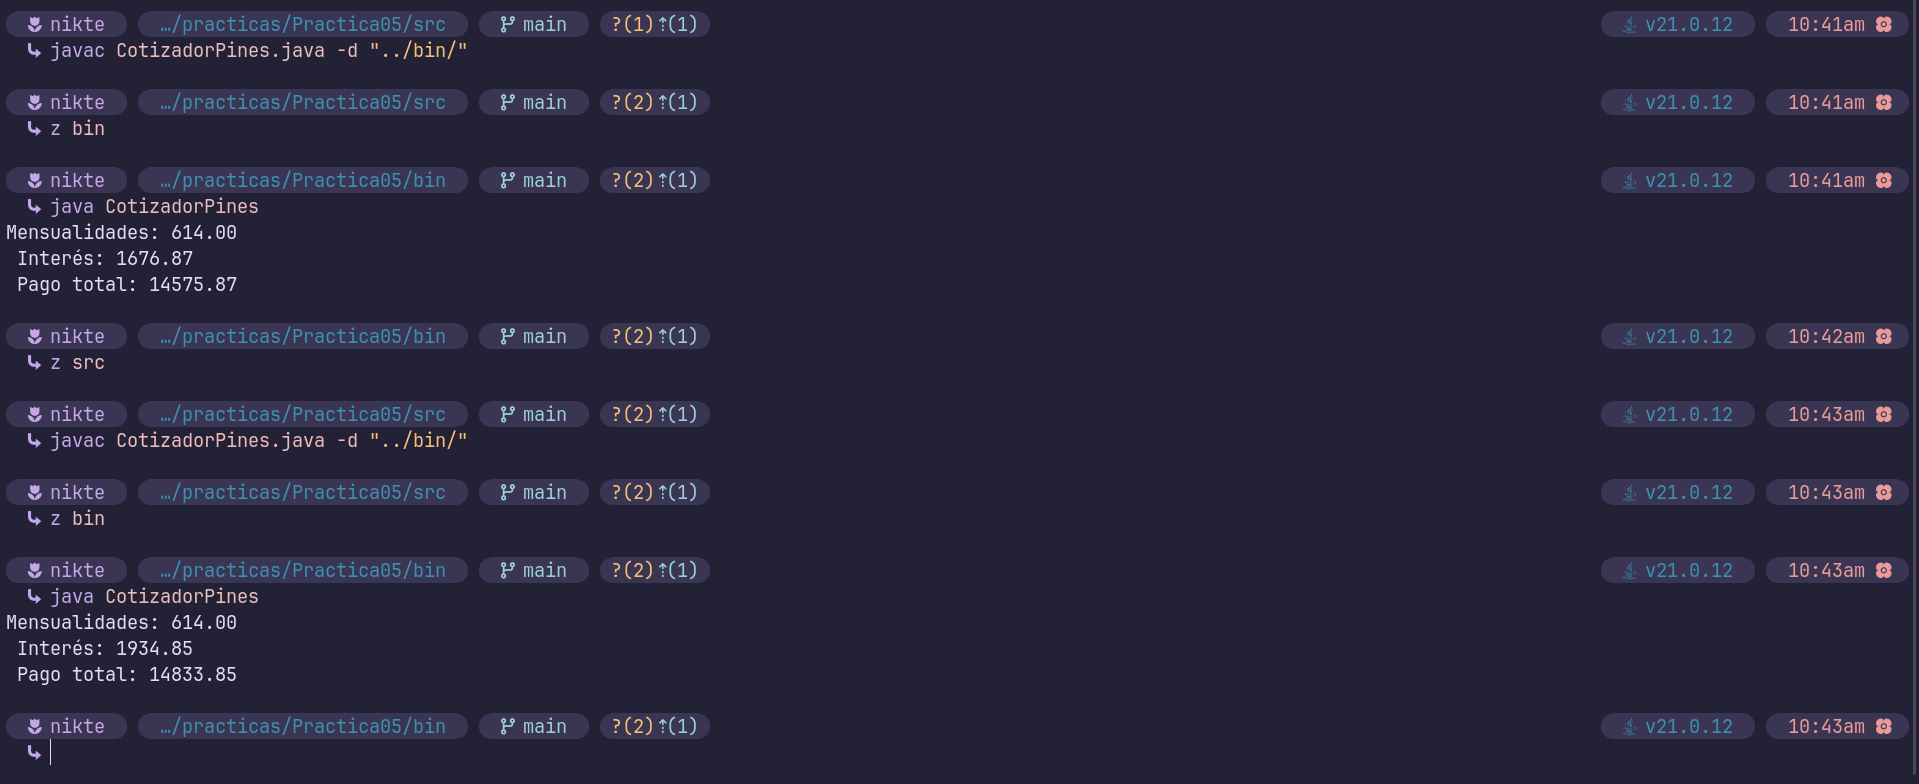
\includegraphics[width=\linewidth]{./images/P2-1-1.png}
			\end{center}

		\subsection*{Actividad 1.2 - Repetir hasta llegar a la precisión deseada}
		
			Para el ejercicio 3 definí una variable que parametrizaba el margen de error permitido, además, definí otra variable en la que se guardaba la estimación del programa, la cual era calculada con el código de la actividad anterior. Se lanzaban más dardos y se actualizaba la estimación, hasta que una variable centinela decía que el margen de error estaba dentro de lo permitido. He de mencionar que, viniendo de Python, asumí que cuando se actualiza una variable, el intérprete automáticamente actualiza \textbf{todas} las variables en las que la variable actualizada se utilice. Grande fue mi sorpresa cuando me dí cuenta de que esto no era así, y era por esto que mis programas nunca dejaban de correr.

			Los resultados de mis ejecuciones fueron:

			\begin{table}[!ht]
			    \centering
			    \begin{tabular}{|l|l|l|l|}
			    \hline
				Tolerancia & Ejecución & Dardos Necesarios & Estimación de $ \pi$ \\ \hline
				0.1 & 1 & 20 & 3.200000 \\ \hline
				0.1 & 2 & 9 & 3.111111 \\ \hline
				0.1 & 3 & 9 & 3.111111 \\ \hline
				~ & ~ & Promedio: 12.66 & ~ \\ \hline
				0.01 & 4 & 60 & 3.133333 \\ \hline
				0.01 & 5 & 93 & 3.139785 \\ \hline
				0.01 & 6 & 70 & 3.142857 \\ \hline
				~ & ~ & Promedio: 74.33 & ~ \\ \hline
				0.001 & 7 & 1080 & 3.140741 \\ \hline
				0.001 & 8 & 247 & 3.141700 \\ \hline
				0.001 & 9 & 205 & 3.141463 \\ \hline
				~ & ~ & Promedio: 510.66 & ~ \\ \hline
			    \end{tabular}
			\end{table}

			Respondiendo las preguntas:

			\begin{itemize}
				\item Bastante, por lo que creo que el promedio no es indicativo de lo que sucede de forma interna en el programa. Como trabaja con números pseudo-aleatorios y las ejecuciones fueron consecutivas, se nota que una pequeña variación en la hora del sistema provoque una mayor utilización de iteraciones, como se ve en la tabla.
				\item Requerí mil dardos, o menos, para obtener una precisión similar a la que el primer programa tuvo con 10 o 100 veces más dardos. Lo que me lleva a pensar que esta implementación explota los rendimientos decrecientes de Monte Carlo porque se detiene cuando cruza una meta, mientas que en la otra implementación, los experimentos adicionales pueden añadir ruido.
			\end{itemize}

			Mi ejecución corrió así (tuve que hacer una nueva porque se me olvidó tomar screenshot la primera vez):

			\begin{center}
				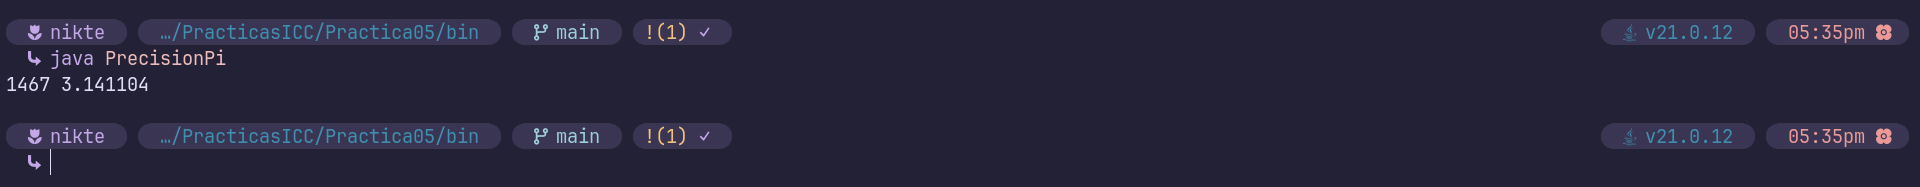
\includegraphics[width=\linewidth]{./images/P1-2-1.png}
			\end{center}

	\section*{Parte 2: El regreso del señor Pines}
		\subsection*{Actividad 2.1 - Verificar los datos y el tipo de cliente}

			Mi programa calcula el interés y préstamo solo si se cumple un booleano que se guarda en una variable llamada \texttt{condicion}. Esta variable es verdadera si tanto la cantidad de meses como el monto del préstamo son mayores a cero. Finalmente, se cambia la tasa del cliente dependiendo de su categoría, si el cliente no entra en ninguna de las dos categorías, por defecto la variable \texttt{condicion} se vuelve falsa y el programa no se ejecuta.

			Mis ejecuciones cambiando al tipo de cliente son estas: se observará que hay un error en los cálculos, porque asumí que la cantidad de años sería entera.
			\begin{center}
				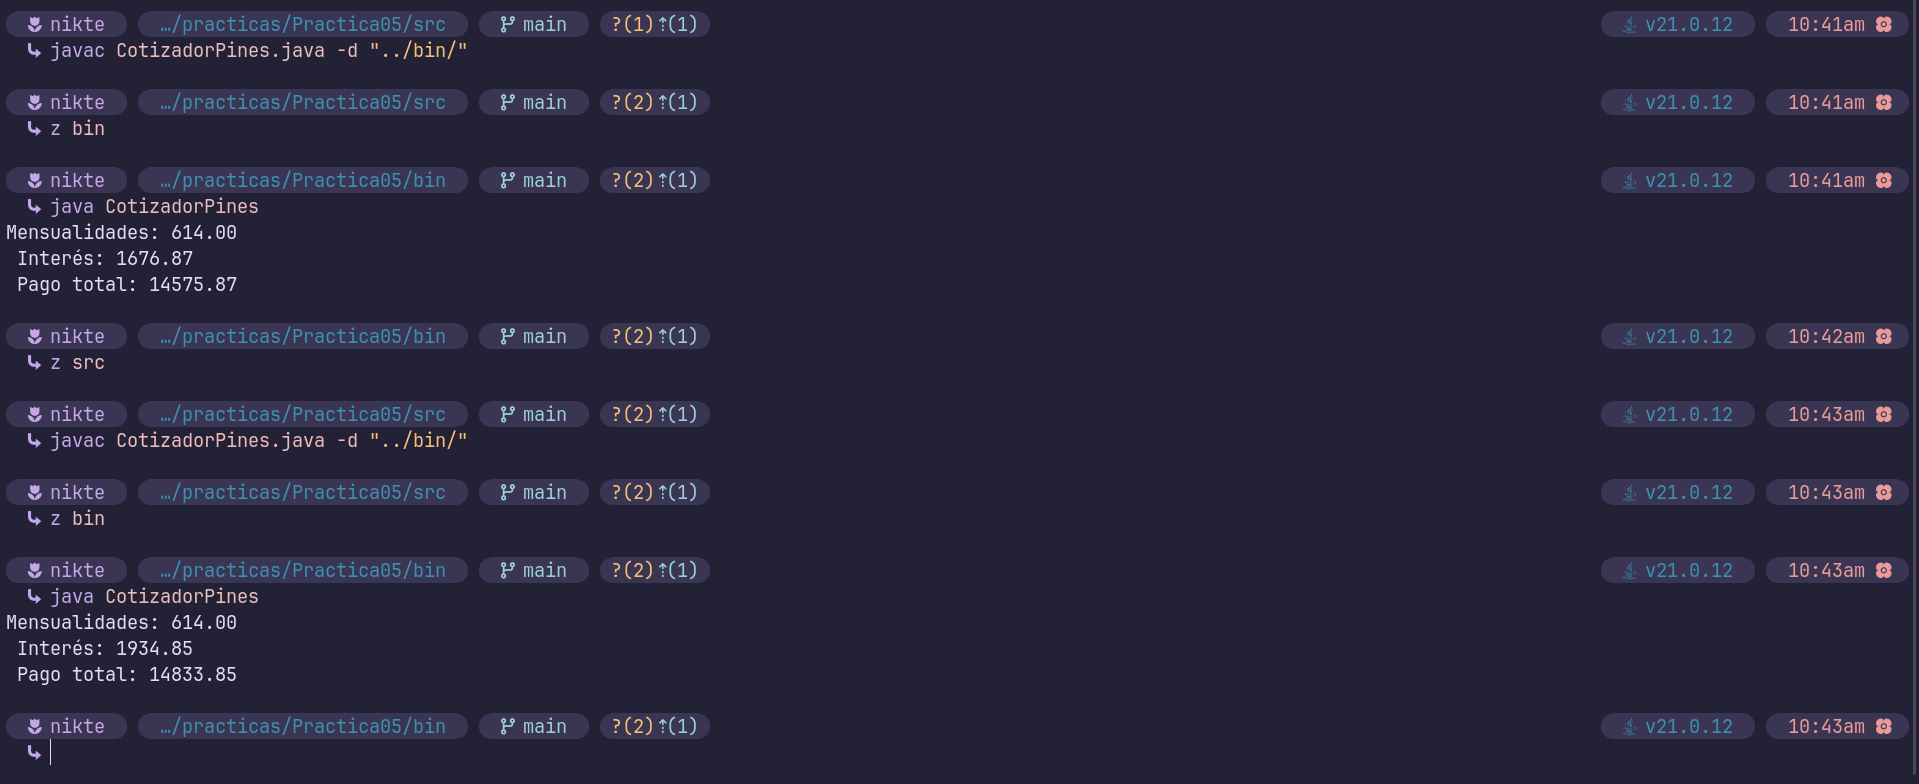
\includegraphics[width=\linewidth]{./images/P2-1-1.png}
			\end{center}

			Mi implementación decía explícitamente cuál era el problema en el programa, para que el cliente no tuviera que estar adivinado cuál era el error:
			\begin{center}
				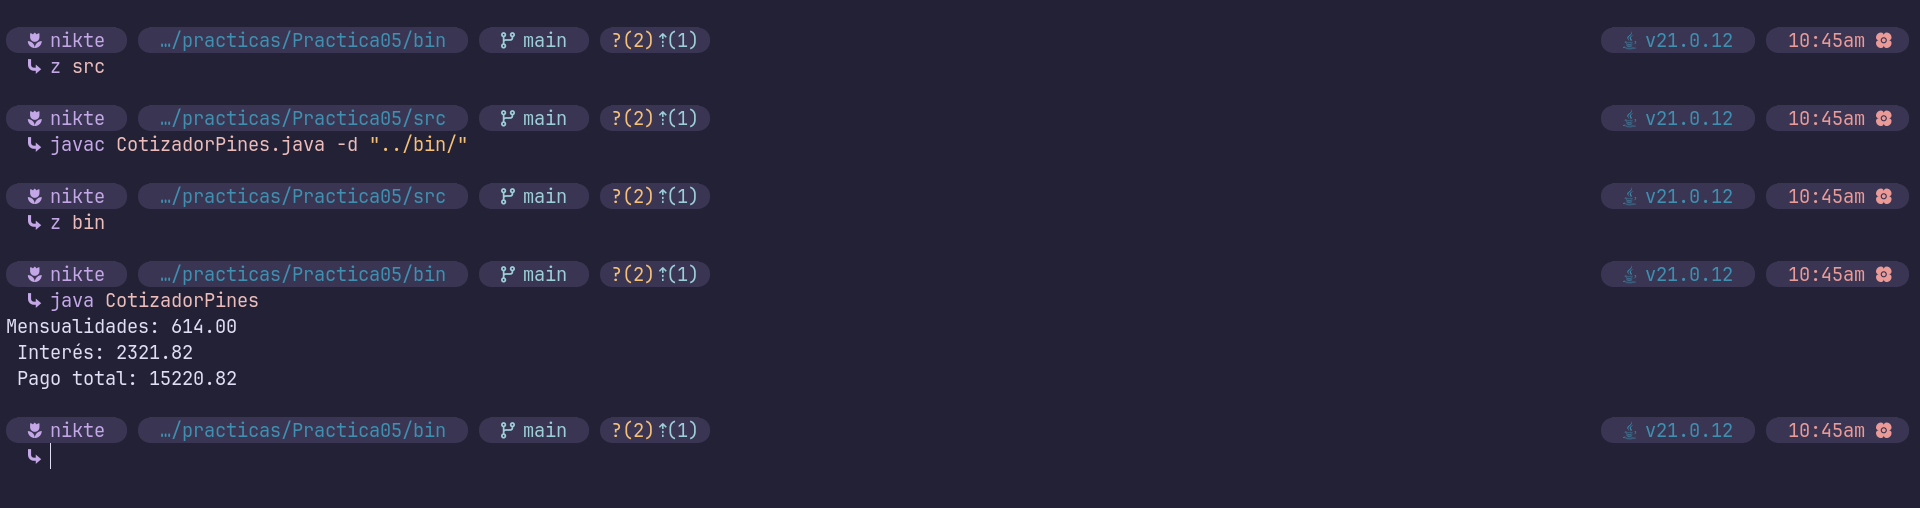
\includegraphics[width=\linewidth]{./images/P2-1-2.png}
			\end{center}
			\begin{center}
				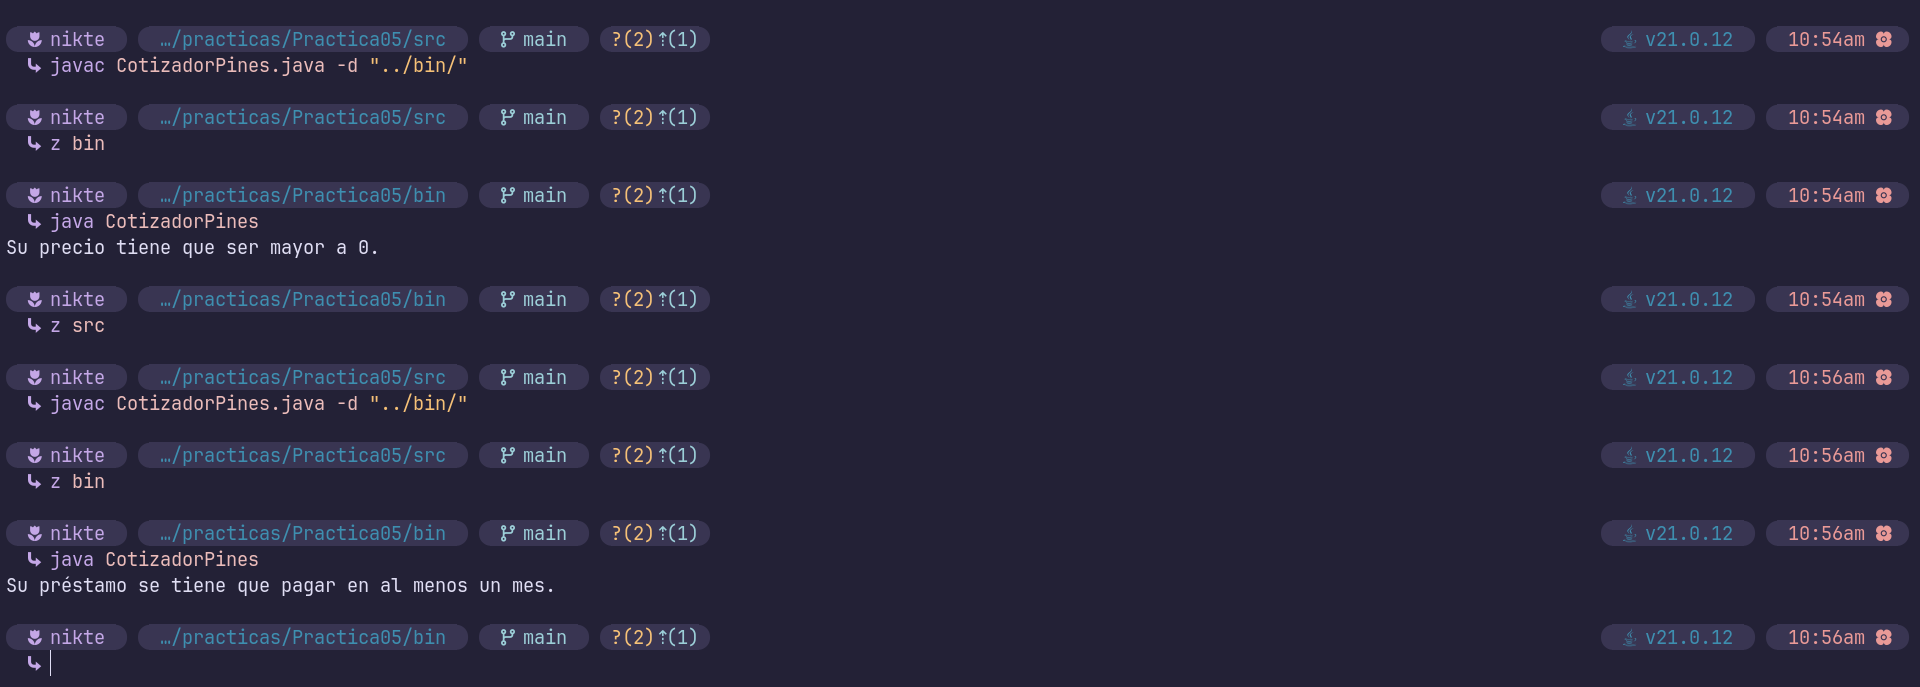
\includegraphics[width=\linewidth]{./images/P2-1-3.png}
			\end{center}

		\subsection*{Actividad 2.2 - Interés compuesto}
			Para resolver esta actividad, utilicé un ciclo \texttt{for} que iteraba sobre los meses. Incidentalmente descubrí que este ciclo debe de iniciar en 1, no en 0, como normalmente se hace, esto es porque una deuda solo se cobra a partir del primer mes. Después, en cada iteración, multiplicaba el saldo por $1+\text{tasa}$ e imprimía el output que se me pedía con \texttt{printf}. Generé también una variable que me decía el interés teórico y la calculé con \texttt{(Math.pow((1+tasaMensual),21))}. El resto fue reutilizar el código anteriormente escrito y explotar \texttt{printf}.

			La captura de que mi programa era correcto:
			\begin{center}
				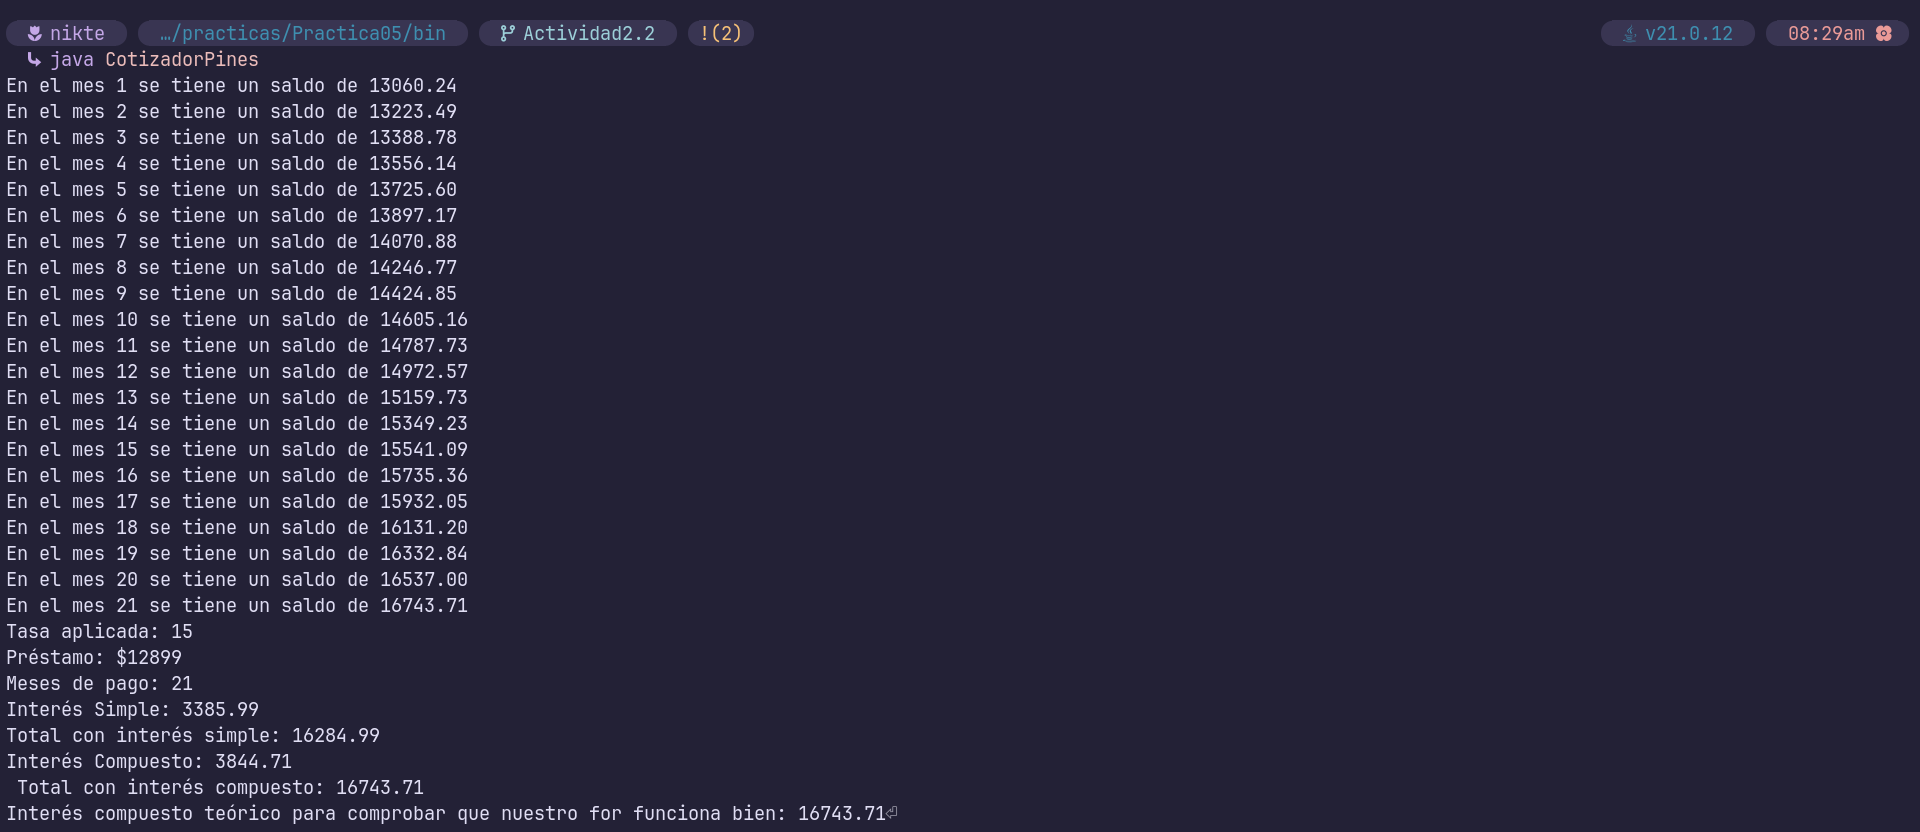
\includegraphics[width=\linewidth]{./images/P2-2-1.png}
			\end{center}
	\section*{Conclusiones}
		Esta práctica me resultó tediosa porque había que poner atención a muchos detalles que normalmente la computadora verifica por mí. Esto motiva la automatización con la programación, cosa que haré de ahora en adelante. Noté que había muchas partes de mi programa que motivaban los conceptos de modularidad y reutilización, justificando muchas de las decisiones del lenguaje de programación Java. El error de lógica con el ciclo \texttt{for} en la actividad 2.2 motiva que, a medida que aprendo diseños de patrones, aplique la máxima de Hamming.

\end{document}
